% !TeX root = ../main.tex
% !TEX root = ../main.tex
% -*- root: ../main.tex -*-
% -*- program: pdflatex -*-
\chapter{双端修正}
上两章主要从插值方法和构造公式入手介绍了对TOF的MRPC的离线数据的刻度方法。研究的主要是单端的刻度。这章将介绍双端刻度方法。

\begin{figure}[!h]
\begin{minipage}[!h]{0.5\linewidth}
%\centering
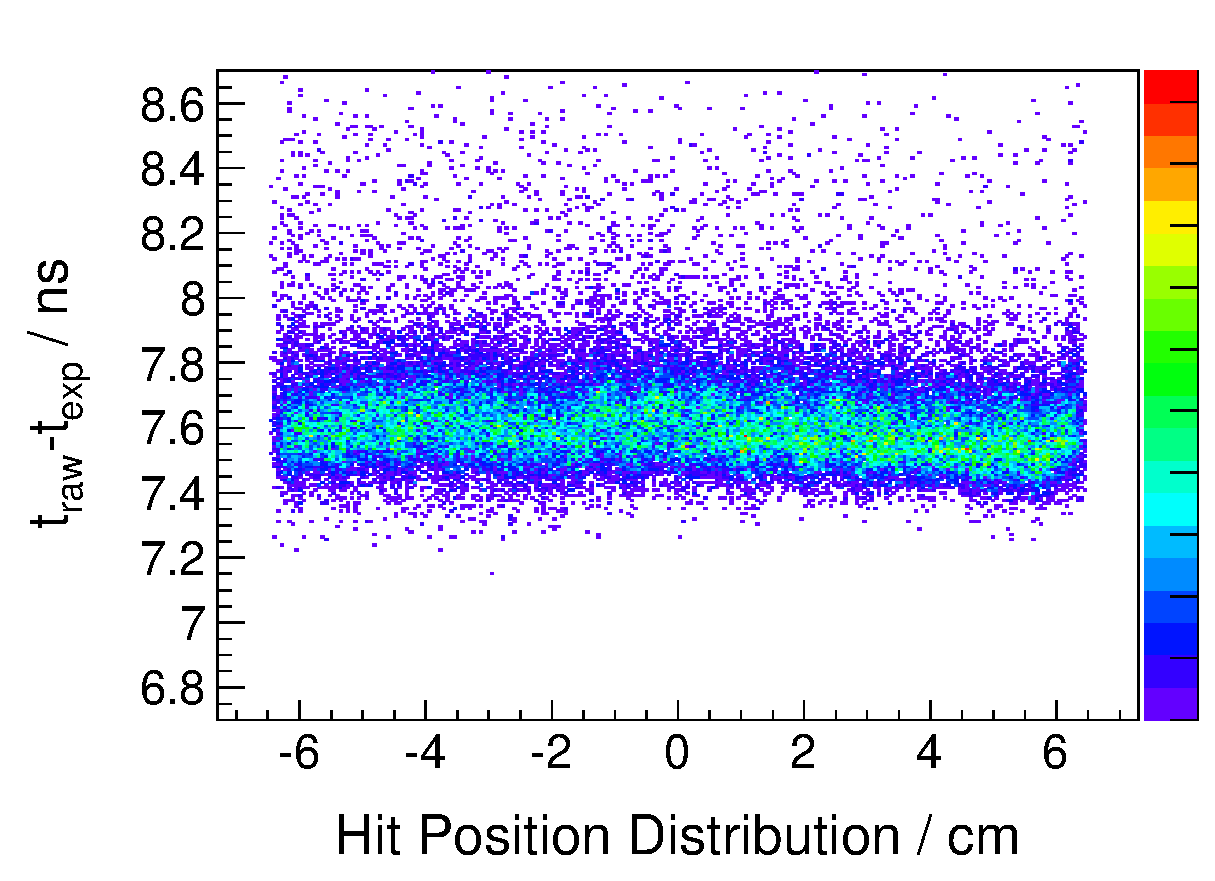
\includegraphics[width=0.9\textwidth]{chap4/combined-tVSz.eps}
\subcaption{双端时间对~Z~的分布}
\label{fig:combined-tVSz}
\end{minipage}%
\hfill
\begin{minipage}[!h]{0.5\linewidth}
%\centering
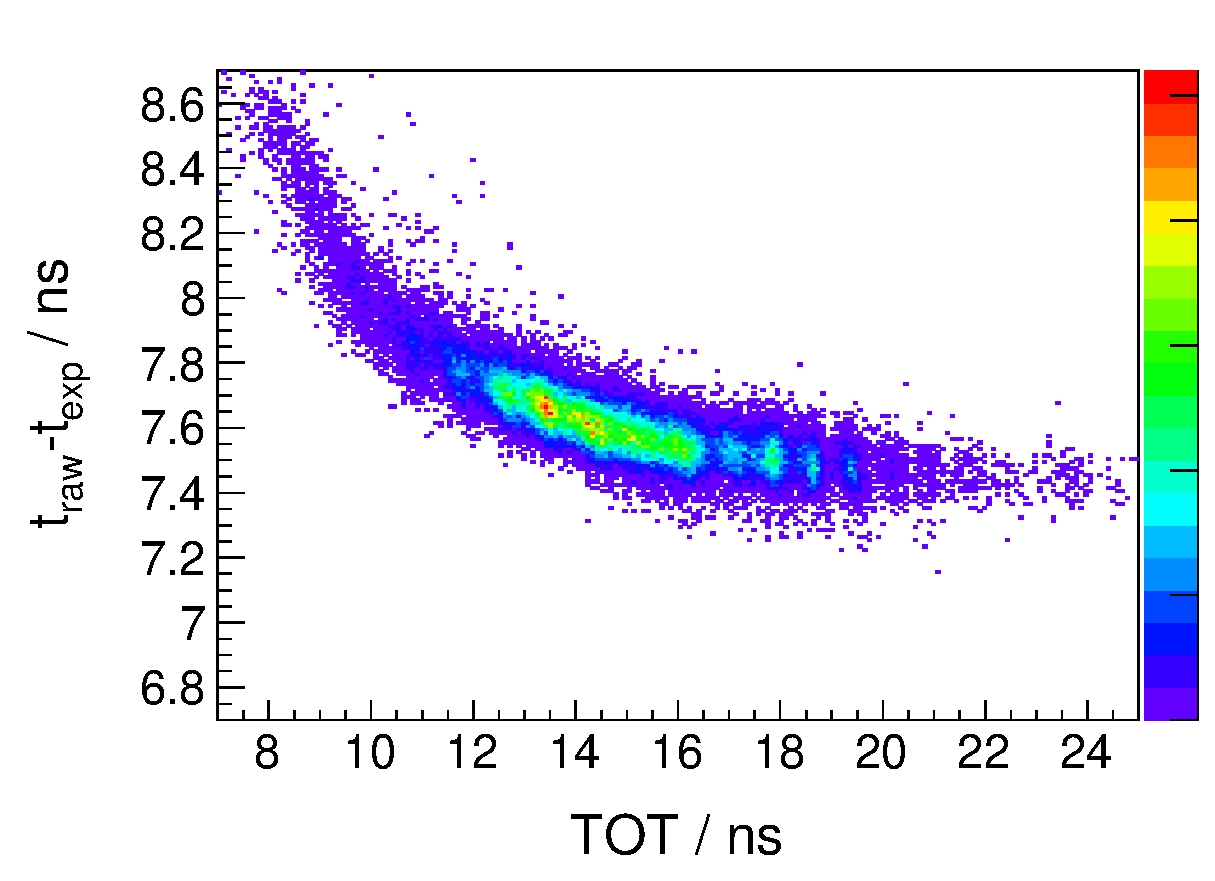
\includegraphics[width=0.9\textwidth]{chap4/combined-tVSq.eps}
\subcaption{时间对~TOT~的分布}
\label{fig:combined-tVSq}
\end{minipage}
\caption{双端时间对~Z~和~TOT~的分布}
\end{figure}

图~\ref{fig:combined-tVSz}~和图~\ref{fig:combined-tVSq}~是双端的时间对~Z~和~TOT~的分布。所谓双端指的是两端时间的平均值,~TOT~采用的也是两端~TOT~的平均值。从图中可以看出,双端的时间对~Z~的依赖很小,主要就是时间对~TOT~的依赖关系。而这时的时间对~TOT~的依赖关系和单端修正~Z~后时间对~TOT~的分布很类似。因此对于双端修正,直接对~TOT~修正,采用和单端修正~Z~后处理时间与~TOT~的关系相同的办法。

\section{双端插值方法}
也是先利用插值方法对双端进行修正。
\section{双端构造公式}
\section{双端对~Z~的修正}
为了绕开径迹外推的信息~zrhit~,采用类似的信息(tleft-tright)/2
\section{小结}












